\documentclass[aspectratio=169,11pt]{beamer}
\usepackage{teaching_slides}

\title[L3 - Linear Regression]{ Econometrics I}
\subtitle{Lecture 2: Linear Regression}
\author{Chris Conlon \\NYU Stern}
\date{Fall 2026}


\begin{document}
\maketitle



\begin{frame}{Linear Regression: Introduction I}
\begin{itemize}
	\item A typical example of a linear regression model:
	\begin{equation*}
		y_i = \beta_1 x_{1,i} +  \beta_2 x_{2,i} + \dots +  \beta_K x_{K,i} + \varepsilon_i,
	\end{equation*}
	where 
	\begin{itemize}
		\item<1-> $i=1,\dots,n$ indexes observations
		\smallskip
		\item<2-> $y_{i}$, a scalar, is often referred to as the {\bf dependent variable}
		\smallskip
		\item<3-> $x_{k,i}$, is the $i$th observation of the $k$th {\bf explanatory variable},
		 or {\bf independent variable} (independent of what?), or  {\bf regressor}
		\smallskip
		\item<4-> The $\beta_{k}$ terms represent the {\bf  parameters}. \\
		There are $K$ parameters, one	for each regressor. Usually $x_{1,i}=1$ (a constant), so $\beta_1$ is the intercept.

		\smallskip
		\item<5-> $\varepsilon_{i}$ is the {\bf disturbance} or {\bf error term}
\smallskip
		\item<6-> Only the $y_{i}$ and $x_{k,i}$ terms are observed by the econometrician.
	\end{itemize}
\end{itemize}
\end{frame}


\begin{frame}{Linear Regression: Introduction II}
\begin{itemize}
	\item A typical example of a linear regression model:
	\begin{equation*}
		y_i = \beta_1 x_{1,i} +  \beta_2 x_{2,i} + \dots +  \beta_K x_{K,i} + \varepsilon_i,
	\end{equation*}
	\item Today's questions: 
	\begin{itemize}
		\item Where does it come from? 
		\item What assumptions do we need to estimate $\boldsymbol{\beta}$?
		\item How do we estimate $\boldsymbol{\beta}$?
		\item How to interpret estimates? 
		\item What are the estimator's finite sample and asymptotic properties? 
	\end{itemize}
\end{itemize}
\end{frame}

\begin{frame}{Linear Regression: Matrix Notation}
	\begin{itemize}
	\item We can express the linear regression model in vector notation
	\begin{equation*}
		{\bf y}= {\bf X} \boldsymbol{\beta} + \boldsymbol{\varepsilon},
	\end{equation*}
	where 
	\begin{itemize}
		\item ${\bf y}$ is an $n\times 1$ vector of observations of the dependent variable
		\item ${\bf X}$ is an $n\times K$ matrix of observations of the regressors
		\item $\boldsymbol{\beta} $ is a $K\times 1$ vector of parameters
		\item $\boldsymbol{\varepsilon}$ is an $n\times 1$ vector of error terms
	\end{itemize}

	\item Note that each row of this equation corresponds to the previous equation for
	a single observation $i$:
	$y_i = {\bf x}_{i}'\boldsymbol{\beta} + \varepsilon_i$,
	where ${\bf x}_i = \left(x_{1,i},\dots,x_{K,i}\right)'$ is $K\times 1$, so ${\bf x}_i'$ is the $i$th row of ${\bf X}$.
\end{itemize}
\end{frame}

\begin{frame}{Notation: Read This Once, Use It All Semester}
\begin{itemize}
	\item Roman symbols are observed, Greek symbols are not.
	\item {\bf Bold lowercase} is a vector, {\bf bold uppercase} is a matrix, plain italic is a scalar.
	\medskip
	\item Subscripts pick out a \emph{piece} of an object, so a subscript never appears on the
	full-sample object itself:
	\begin{center}
	\begin{tabular}{lll}
	\hline
	Symbol & Size & What it is \\
	\hline
	${\bf y}$ & $n\times 1$ & all $n$ outcomes \\
	$y_{i}$ & scalar & outcome for observation $i$ \\
	${\bf X}$ & $n\times K$ & all the data on all $K$ regressors (column 1 is usually ones) \\
	${\bf x}_{i}$ & $K\times 1$ & all $K$ regressors for observation $i$ (row $i$ of ${\bf X}$, transposed) \\
	$x_{k,i}$ & scalar & regressor $k$ for observation $i$ \\
	\hline
	\end{tabular}
	\end{center}
	\medskip
	\item So ${\bf X}_{i}$ and ${\bf e}_{i}$ are never things. Watch for this in your own work.
\end{itemize}
\end{frame}

\begin{frame}{Example: Mincerian Regression I}
\begin{itemize}
	\item Let's suppose we are interested in how worker's wages depend on education and experience
	(known as Mincerian regression or Mincer earnings function for Jacob Mincer).

	\medskip
	\item $y_{i}$ could be worker $i$'s wages, and ${\bf x}_i' = \left(1,\text{edu}_i,\text{exp}_i \right)$, 
	where 
	\begin{itemize}
		\item $\text{edu}_i$ is worker $i$'s education (in years)
		\item $\text{exp}_i$ is worker $i$'s work experience (in years)
		\item Note that the regressors include a constant 
	\end{itemize}
\end{itemize}
\end{frame}

\begin{frame}{Example: Mincerian Regression II}
\begin{itemize}
	\item $y_{i}$ is $i$'s wages, and ${\bf x}_i' = \left(1,\text{edu}_i,\text{exp}_i \right)$

	\medskip
	\item The data matrices for the Mincerian regression might look like this:
\[
{\bf y}=\left(\begin{array}{c}
12\\
35\\
20\\
\vdots
\end{array}\right)\qquad\qquad{\bf X}=\left(\begin{array}{ccc}
1 & 12 & 2\\
1 & 16 & 5\\
1 & 12 & 21\\
\vdots & \vdots & \vdots
\end{array}\right)
\]
\end{itemize}
\end{frame}

\begin{frame}{Strict Exogeneity}
	\begin{equation*}
		{\bf y}= {\bf X} \boldsymbol{\beta} + \boldsymbol{\varepsilon}
	\end{equation*}
\begin{itemize}
	\item This equation doesn't mean much until we say something about the error term $\boldsymbol{\varepsilon}$.

	\item The first (and strongest) assumption on error terms we will consider is {\bf strict exogeneity}:\[
		\E\left[\boldsymbol{\varepsilon} | {\bf X} \right] = {\bf 0}
	\]

	\item Note that the law of iterated expectations implies\[
		\E\left[\varepsilon_i\right] = \E_{{\bf X}} \left[\E\left[\varepsilon_i | {\bf X}\right] \right] = 0.
	\]
	It also implies that each error term is uncorrelated with every regressor for every observation: $\Cov\left[\varepsilon_{i},x_{k,j}\right]=0$ 
	for all $i,j,k$ (in particular, $\Cov\left[\varepsilon_{i}, {\bf x}_{i}\right]={\bf 0}$).
\end{itemize}
\end{frame}


\begin{frame}{Strict Exogeneity and Conditional Means}
\begin{align*}
{\bf y} & =  {\bf X}\boldsymbol{\beta}+\boldsymbol{\varepsilon}	& (1)\\
\E\left[\boldsymbol{\varepsilon}|{\bf X}\right] & =  {\bf 0}						& (2)
\end{align*}
\begin{itemize}
	\item Now, we have a meaningful model. 
	\item Note that
\begin{align*}
\E\left[{\bf y}|{\bf X}\right] & =  \E\left[{\bf X}\boldsymbol{\beta}+\boldsymbol{\varepsilon}|{\bf X}\right]\\
 & =  {\bf X}\boldsymbol{\beta}+\E\left[\boldsymbol{\varepsilon}|{\bf X}\right]\\
 &  = {\bf X}\boldsymbol{\beta},
\end{align*}
so equations (1) and (2) already imply that the conditional mean is a linear function of ${\bf X}$.
\end{itemize}
\end{frame}

\begin{frame}{Strict Exogeneity Interpretation}
\begin{align*}
{\bf y} & =  {\bf X}\boldsymbol{\beta}+\boldsymbol{\varepsilon}	& (1)\\
\E\left[\boldsymbol{\varepsilon}|{\bf X}\right] & =  {\bf 0}						& (2)
\end{align*}
\begin{itemize}
	\item Strict exogeneity captures the idea that $x$ is varied in the data without changing the mean
	of the unobservable factors affecting $y$. 

	\medskip
	\item Strict exogeneity is very plausible in the context of experimental variation (especially in double blind studies) 

	\medskip
	\item Unfortunately, social scientists are often unable to rely on experimental variation, and strict exogeneity 
	is rarely plausible in the context of naturally occurring data. For this reason, in future lectures we will consider
	different identification assumptions, but strict exogeneity is a starting point.
\end{itemize}
\end{frame}


\begin{frame}{Omitted Variables and Endogeneity}
\begin{itemize}
	\item Suppose we estimate the following Mincerian regression:\[
\ln \left(\text{wage}_{i}\right)=\beta_{0}+\beta_{1}\text{edu}_{i}+\beta_{2}\text{exp}_{i}+\beta_{3}\text{exp}_{i}^{2}+\varepsilon_{i}.
\]

	\item Furthermore suppose the true model is:\[
\ln \left(\text{wage}_{i}\right)=\beta_{0}+\beta_{1}\text{edu}_{i}+\beta_{2}\text{exp}_{i}+\beta_{3}\text{exp}_{i}^{2}+ \textcolor{red}{\beta_4 \text{ability}_{i}} + \varepsilon_{i}
\]

	\item Then, when estimating the first equation (because ability is unobserved), the error term is effectively:\[
	\widetilde{\varepsilon}_{i} = \beta_4 \text{ability}_{i} + \varepsilon_{i}
\]


\item Note that even if $\varepsilon_{i}$ satisfies strict exogeneity, $\widetilde{\varepsilon}_{i}$ will not
 	if, for instance, ability is correlated with education. We say $x$ is {\bf endogenous} if $\E\left[\varepsilon|x\right]\ne 0$.


\end{itemize}
\end{frame}



\begin{frame}{Wherefore Linearity?}
\begin{itemize}
	\item When would $\E\left[y_i|{\bf x}_i\right] = {\bf x}_i'\boldsymbol{\beta}$ be true?

	\medskip
	\item We might start with the conditional mean as a general function of ${\bf x}_i$\[
	 y_{i} = f\left({\bf x}_{i}\right)+\varepsilon_{i},
	\]
	and then what we've done is impose that $f$ is a linear function. 

		\medskip
	\item We might also think of the model as a linear approximation (using Taylor's theorem). 
	\begin{itemize}
		\item Actually, it can be a polynomial approximation, not just a linear approximation \dots
	\end{itemize}
\end{itemize}
\end{frame}

% example of nonlinear model: Michaelis-Menten model of enzyme kinetics

\begin{frame}{Linear-in-Parameters I}
\begin{itemize}
	\item The linear regression framework does not impose that $y$ is a linear function of any
	particular variable $x$

	\medskip
	\item The regressors in ${\bf x}_i$ can include squared terms, higher powers, and other functions of 
	a variable $x$

	\medskip
	\item For example, ${\bf x}_i' = \left(1,\text{edu}_i,\text{exp}_i,\text{exp}_i^2\right)$ in the Mincerian regression would allow
	declining (or increasing) returns to work experience. 

	\medskip
	\item The ``Linear'' part of ``Linear Regression'' really means linear-in-parameters, which is much less
	 restrictive than being linear with respect to a particular variable.
\end{itemize}
\end{frame}

\begin{frame}{Linear-in-Parameters II}
\begin{itemize}
	\item The dependent variable can also involve nonlinear transformations.

	\smallskip	
	\item For example, $y_{i}$ in the Mincerian regression is typically the natural log of worker $i$'s wage:\[
\ln \left(\text{wage}_{i}\right)=\beta_{0}+\beta_{1}\text{edu}_{i}+\beta_{2}\text{exp}_{i}+\beta_{3}\text{exp}_{i}^{2}+\varepsilon_{i}.
\]

	\smallskip
	\item Models of demand (or supply) sometimes have the form\[
		\ln \left( q_{i} \right) = \beta_0 + \beta_1 \ln \left( p_{i}\right) + \varepsilon_i,
	\]
	in which case $ \beta_1$ represents the price elasticity of demand (supply) and does not depend on the units that prices
	and quantities are measured in  (Check this). Economists love logs!
	

	\smallskip
	\item What would it take for a model to not be linear in parameters?

	\smallskip
	\item Much more on \alert{why} we transform $y$ and $x$ (logs, elasticities,
	odds, rare events) in the companion deck: \emph{Lecture 2b: Transformations}.
\end{itemize}
\end{frame}

\begin{frame}{Derivation from Multivariate Normal}
\begin{itemize}
	\item Another way to motivate the linear regression function is from the multivariate normal distribution.

	\smallskip
	\item Suppose $\left(y,x\right)' \sim \mathcal{N}\left(\boldsymbol{\mu},\boldsymbol{\Sigma}\right)$, where\[
\boldsymbol{\mu}=\left(\begin{array}{c}
\mu_{y}\\
\mu_{x}
\end{array}\right)\qquad\qquad\boldsymbol{\Sigma}=\left(\begin{array}{cc}
\sigma_{y}^{2} & \rho\sigma_{y}\sigma_{x}\\
\rho\sigma_{y}\sigma_{x} & \sigma_{x}^{2}
\end{array}\right)
\]


\end{itemize}
\end{frame}



  \begin{frame}
\frametitle{Multivariate Normal Data}
\begin{columns}
\begin{column}{0.4\textwidth}
\[
\boldsymbol{\mu}=\left(\begin{array}{c}
0\\
0
\end{array}\right)
\]

\[
\boldsymbol{\Sigma}=\left(\begin{array}{cc}
4 & -1\\
-1 & 1
\end{array}\right)
\]
\end{column}
\begin{column}{0.6\textwidth} 
    \begin{center}
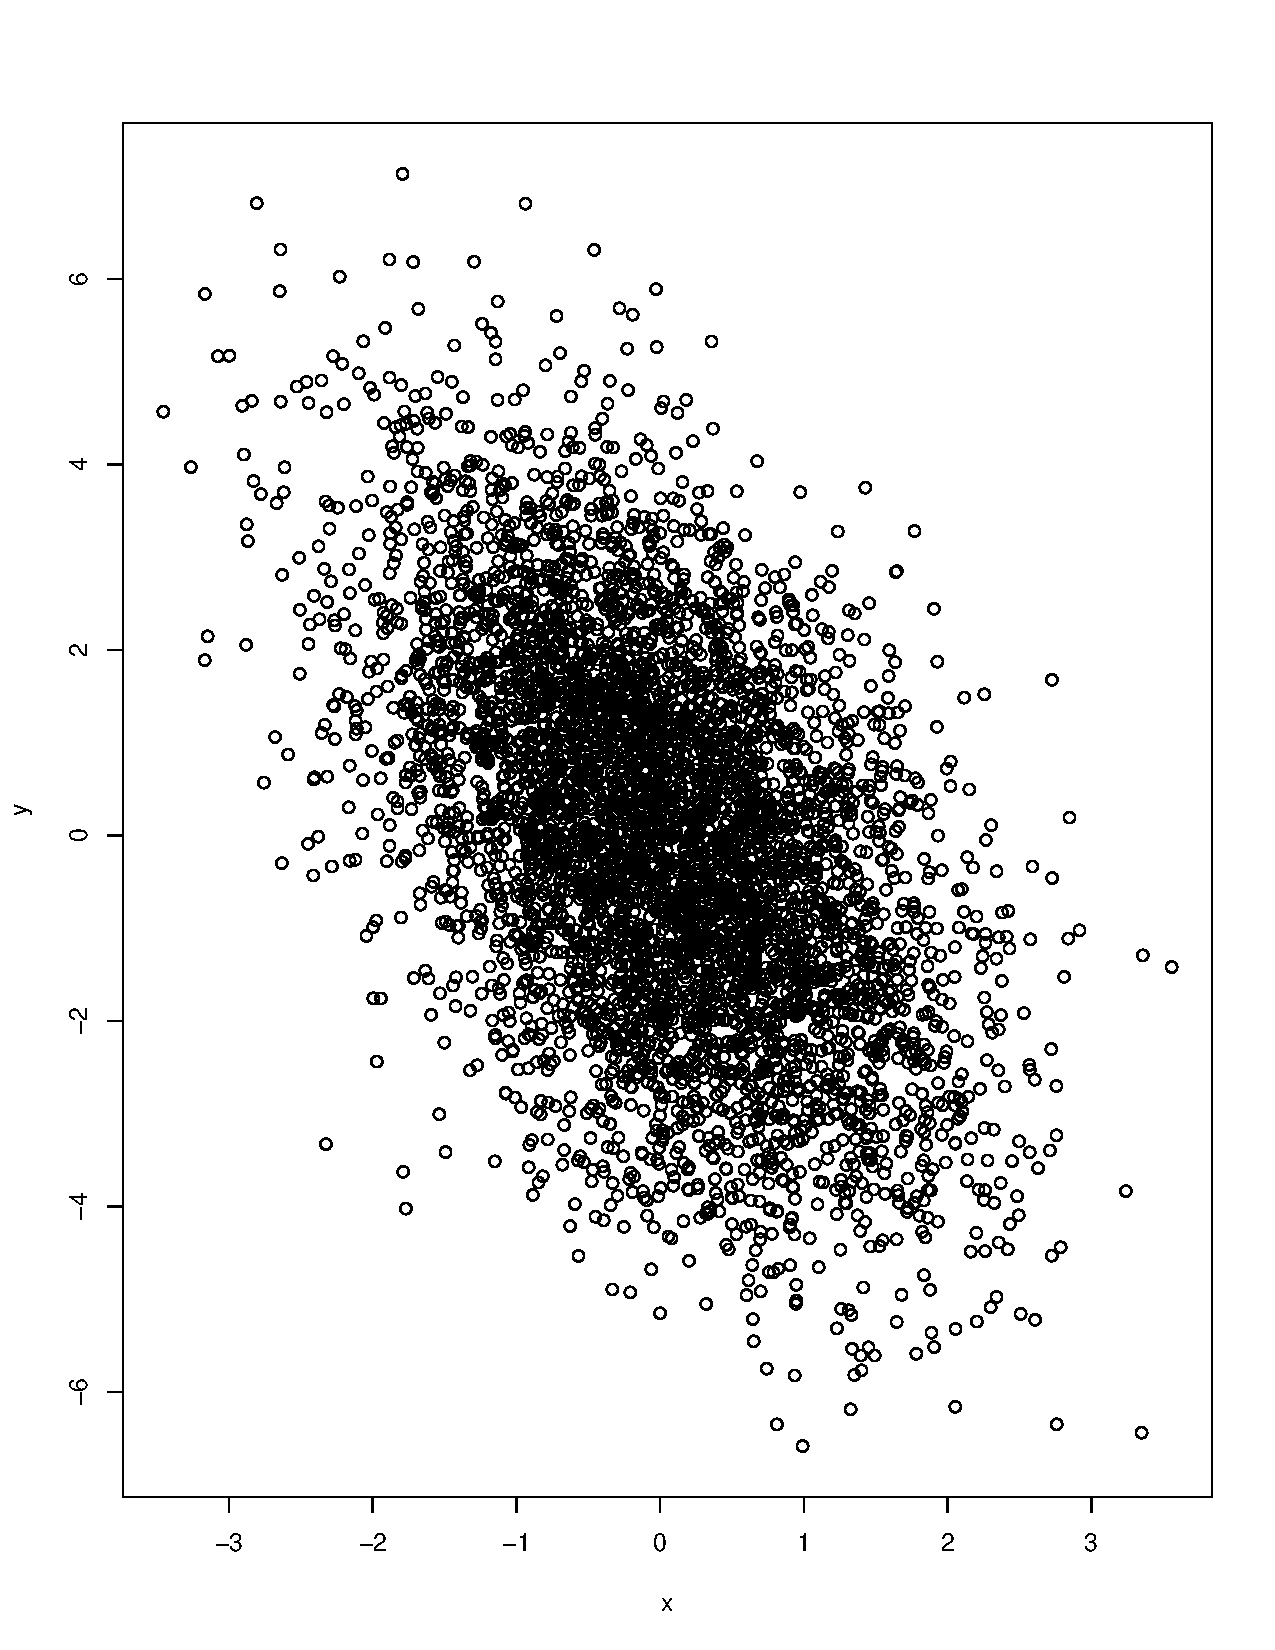
\includegraphics[width=.8\textwidth]{mvnormal_scatter.pdf}
     \end{center}
\end{column}
\end{columns}
\end{frame}


%  \begin{frame}
%\frametitle{Multivariate Normal Marginal Densities}
%\begin{center}
%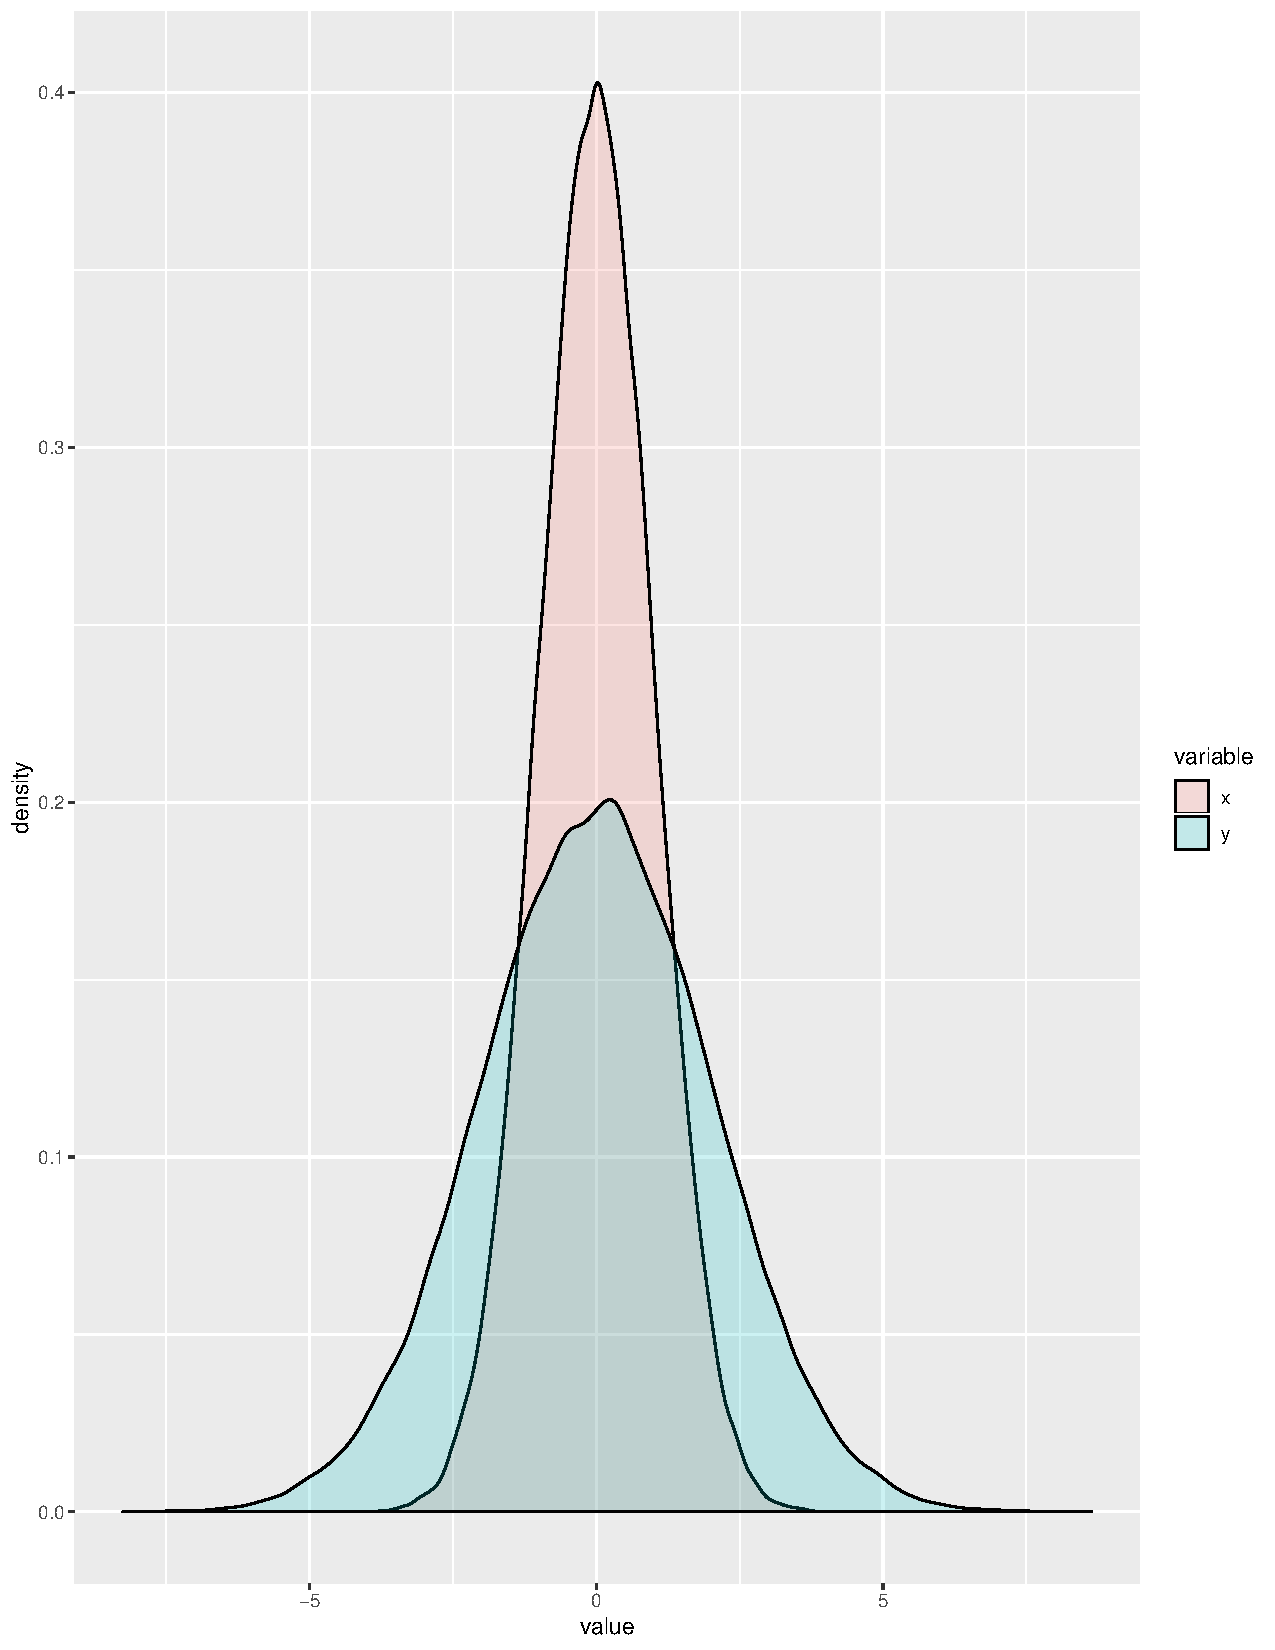
\includegraphics[scale=.25]{marginal_dists.pdf}
%\end{center}
%\end{frame}

 % \begin{frame}
%\frametitle{Multivariate Normal Marginal Densities}
%\begin{center}
%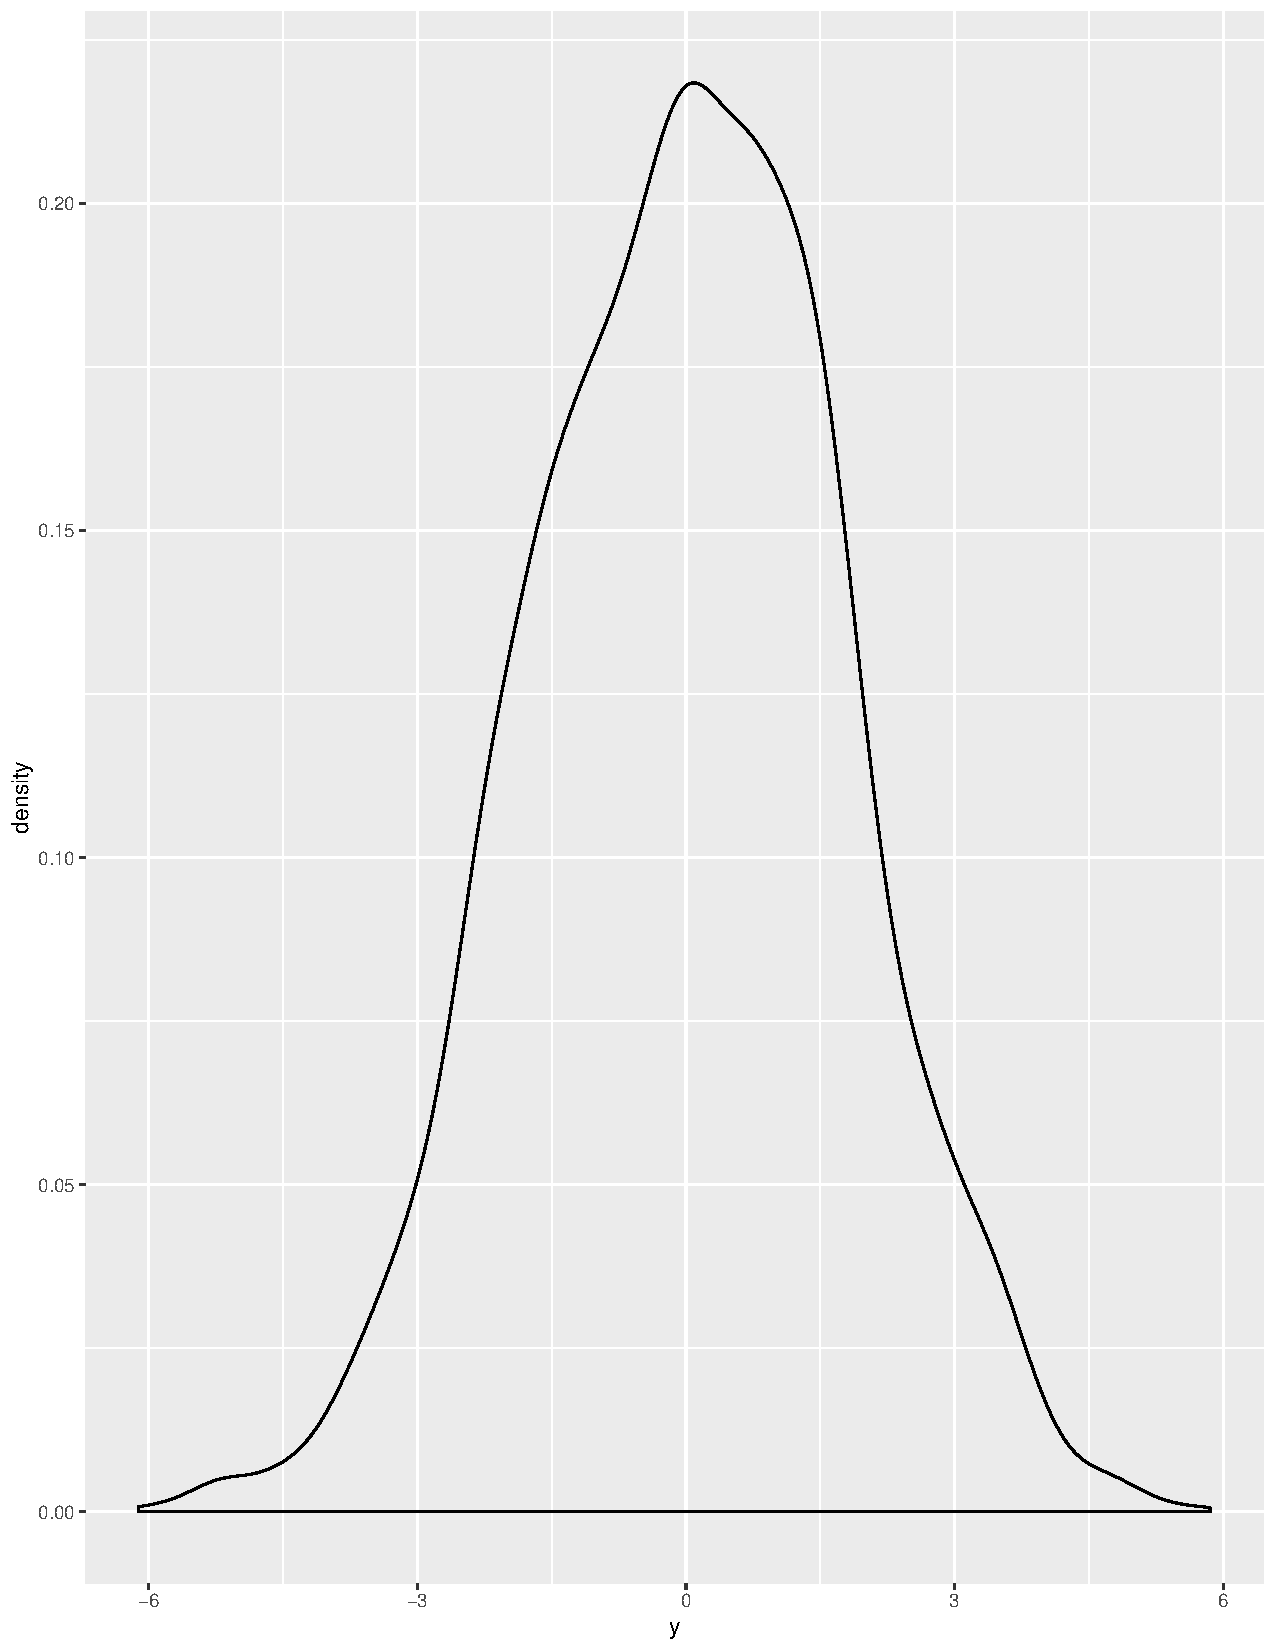
\includegraphics[scale=.2]{cond_dist.pdf}
%\end{center}
%\begin{itemize}
%	\item Here, I approximate the conditional density
%	$Pr\left(y|x=0\right)$ by plotting the density of $y$
%	when we focus on observations with $x\in\left(-.04,.04\right)$
%\end{itemize}
%\end{frame}


\begin{frame}[fragile]{ R code}
\begin{lstlisting}
# install.packages('MASS')
# install.packages('ggplot2')
# install.packages('reshape')
library(MASS)
library(ggplot2)
library(reshape)

mu <- c(0,0)
Sigma <- matrix(c(1,-1,-1,4),2,2)
xy <- mvrnorm(n = 5000, mu, Sigma)
plot(xy, xlab="x",ylab="y")

xy <- mvrnorm(n = 100000, mu, Sigma)
xy.df <- as.data.frame(xy)
names(xy.df) <- c("x", "y")
xy.stacked <- melt(xy.df)
ggplot(xy.stacked, aes(value, fill = variable)) + geom_density(alpha = 0.2)

xy.selected <- xy.df[xy.df$x>-.04  & xy.df$x<.04, ]
ggplot(xy.selected, aes(y)) + geom_density(alpha = 0.2)
\end{lstlisting}
\end{frame}


\begin{frame}{Multivariate Normal and Regression Equation}
\begin{itemize}

	\item Suppose $\left(y,x\right)' \sim \mathcal{N}\left(\boldsymbol{\mu},\boldsymbol{\Sigma}\right)$, where \[
\boldsymbol{\mu}=\left(\begin{array}{c}
\mu_{y}\\
\mu_{x}
\end{array}\right)\qquad\qquad\boldsymbol{\Sigma}=\left(\begin{array}{cc}
\sigma_{y}^{2} & \rho\sigma_{y}\sigma_{x}\\
\rho\sigma_{y}\sigma_{x} & \sigma_{x}^{2}
\end{array}\right)
\]

	\smallskip
	\item It's also the case that \[
		\E\left[y|x\right] = \mu_y + \rho\frac{\sigma_y}{\sigma_x}\left(x-\mu_x\right)
	\]
	and \[
		y = \E\left[y|x\right] + \varepsilon, \qquad \varepsilon \sim \mathcal{N}\left(0,\sigma_y^2\left(1-\rho^2\right)\right) \text{ independent of } x.
	\]

	\smallskip
	\item Normally distributed error terms: the first case we will consider (and easiest to analyze)

\end{itemize}
\end{frame}


\begin{frame}{Full Rank I}
\begin{itemize}

	\item<1-> Our next assumption is that the matrix of regressors has {\bf full rank}
	\begin{itemize}
		\item<1-> ${\bf X}$ is a $n\times K$ matrix with rank $K$.
	\end{itemize}

	\medskip
	\item<2-> A model of consumption that violates full rank:\[ 
	C = \beta_1 + \beta_2 \text{Salary} + \beta_3 \text{Nonsalary income} + \beta_4 \text{Total income} + \varepsilon
	\]

	\medskip
	\item<3-> Conditional on total income, any increase in salary must be met by an equal decrease
	in nonsalary income

%	\medskip
%	\item<3-> Suppose we knew $\beta_4$ -- how would we be able to determine $\beta_2$ and $\beta_3$? 

\end{itemize}
\end{frame}

\begin{frame}{Full Rank II}
\begin{itemize}

	\item Consider the following model of consumption:\[ 
	C = \beta_1 + \beta_2 \text{Salary} + \beta_3 \text{Nonsalary income} + \beta_4 \text{Total income} + \varepsilon
	\]
	\smallskip
\[
	\text{Total income}  = \text{Salary} + \text{Nonsalary income},
	\]
	so\[
\begin{array}{ccl}
C & = & \beta_{1}+\left(\beta_{2}+\beta_{4}\right)\text{Salary}+\left(\beta_{3}+\beta_{4}\right)\text{Nonsalary income}+\varepsilon\\
C & = & \beta_{1}+\widetilde{\beta}_{2}\text{Salary}+\widetilde{\beta}_{3}\text{Nonsalary income}+0\cdot\text{Total income}+\varepsilon
\end{array}
\]

	\smallskip
	\item Assuming $\beta_{4}\ne 0$ in the original equation, we have constructed an empirically equivalent equation with different parameters.
         That is, for this model, we have different values for $\boldsymbol{\beta}$ that are {\bf observationally equivalent}. 

\end{itemize}
\end{frame}


\begin{frame}{Full Rank III}
\begin{itemize}

	\item Exercise: suppose I wanted to build a model of the approval ratings of major party nominees 
	for US president. 

	\item I want to include the following regressors:
	\begin{itemize}
		\item Years holding elected office
		\item Age
		\item Gender
		\item Indicator variable for being married to a former president
	\end{itemize}

	\item What's the problem, assuming I have data through 2020? What about in 2025? \\ Compare to the previous case with salaries -- any difference? 



\end{itemize}
\end{frame}

\begin{frame}{Linear Independence}
\begin{itemize}

	\item Another term for the full rank assumption ($\operatorname{rank}\left({\bf X}\right)=K$) is {\bf linear independence}.
	 {\bf Multicollinearity} refers to a lack of linear independence. When a model has multicollinearity, we 
  	say it is {\bf not identified}. 

	\medskip
	\item Note that this is distinct from statistical independence. 

	\medskip
	\item Linear independence means that one variable cannot be algebraically predicted by others. 

	\medskip
	\item Statistical independence means that the variation in two random variables is unrelated.
	Linear independence does not imply statistical independence. Why not? Does statistical independence
	imply linear independence? 
\end{itemize}
\end{frame}


\begin{frame}{Assumptions so far}
\begin{itemize}
	\item The assumptions we have introduced so far:
\end{itemize}

\begin{align*}
{\bf y} & =  {\bf X}\boldsymbol{\beta}+\boldsymbol{\varepsilon}	& (1)\\
\E\left[\boldsymbol{\varepsilon}|{\bf X}\right] & =  {\bf 0}						& (2) \\
\operatorname{rank}({\bf X}) & = K 	& (3)
\end{align*}

\begin{itemize}
	\item Note that we have not made any assumptions on the statistical properties of ${\bf X}$.
	There is no need to do so; ${\bf X}$ can be fixed or random \emph{for now}. What matters
	is the distribution of the error terms conditional on  ${\bf X}$.

	\item Not all assumptions will be maintained throughout the course (or even this lecture).
	When we consider formal results, I will be explicit about which assumptions are needed. 
	
\end{itemize}
\end{frame}

\begin{frame}{Homoscedasticity}
\begin{itemize}
	\item Another important assumption is {\bf homoscedasticity}:\[
		\E\left[\boldsymbol{\varepsilon} \boldsymbol{\varepsilon}' | {\bf X} \right] = \sigma^{2} {\bf I}
	\]
	where ${\bf I}$ is the $n \times n$ identity matrix.

	\medskip
	\item Given that $\E\left[\boldsymbol{\varepsilon}|{\bf X}\right] =  {\bf 0}$, this means that\[
	\Var\left[\boldsymbol{\varepsilon} | {\bf X} \right] = \sigma^{2} {\bf I}
	\]

	\item In words, homoscedasticity says that each error term has the same variance; i.e.,   
	the variance of $\varepsilon_i$ is not related to ${\bf x}_i$. {\bf Heteroscedasticity}
	is the alternative. Can you think of some cases of heteroscedasticity? 

	\item The assumption also rules out correlation between the error terms for different observations.
	
\end{itemize}
\end{frame}



\begin{frame}{Normal Error Terms}
\begin{itemize}
	\item A convenient assumption 
	 is that error terms are {\bf normally distributed}:\[
		\boldsymbol{\varepsilon} | {\bf X} \sim \mathcal{N}\left({\bf 0},\sigma^2 {\bf I}\right)
	\]

	\medskip
	\item Where are we going?
	\begin{itemize}
		\item This assumption will make it easy to derive normally distributed estimators (just as
			normality made the LLN and CLT easy to derive)
		\item Ultimately, the central limit theorem can be used to derive {\bf asymptotic normality}
				of estimators (that is, estimators that will be normally distributed as the sample gets large),
				so in practice it's rarely necessary to assume normal error terms. 
	\end{itemize}

\end{itemize}
\end{frame}



\begin{frame}{Residuals}
\begin{itemize}
	\item We used $\boldsymbol{\beta}$ to denote the true vector of parameters; let's use
	${\bf b}$ to denote estimates of or candidates for $\boldsymbol{\beta}$.

	\item A residual is the gap between $y_i$ and its fitted value under a candidate parameter vector ${\bf b}$:\[
		e_i \left({\bf b}\right) = y_i - {\bf x}_i' {\bf b}
	\]

	\item A residual captures the part of the dependent variable $y_{i}$ that the linear prediction ${\bf x}_i' {\bf b}$
	fails to explain.
	

	\item Formally, we should think of residuals as being a function of candidate parameter
	vectors, but we will often just write $e_i$. 


	\item The vector of residuals across observations is ${\bf e} \left({\bf b}\right)$
\end{itemize}
\end{frame}


\begin{frame}{Least Squares}
\begin{itemize}
	\item It makes intuitive sense to want to find a value of ${\bf b}$
	 that makes residuals small, so that the estimated model explains the data well.

	\smallskip
	\item There are many possible ways to think about making the residuals small, but
	by far the most popular criterion is the {\bf sum of squared residuals}:\[
		SSR\left({\bf b}\right) \equiv \sum_{i=1}^{n} e_i \left({\bf b}\right)^2  =  \sum_{i=1}^{n} \left(y_i - {\bf x}_i' {\bf b}\right)^{2} = {\bf e} \left({\bf b}\right) '  {\bf e} \left({\bf b}\right)
	\]

	\smallskip
	\item The {\bf least squares estimator} minimizes the sum of squared residuals:\[
		{\bf b}_{LS} \equiv \argmin_{{\bf b}} SSR\left({\bf b}\right) 
	\]

	\smallskip
	\item For linear models with homoscedastic errors, the least squares estimate is typically called the
	{\bf Ordinary Least Squares} estimator.

\end{itemize}
\end{frame}



\begin{frame}{Regression with Single Variable I}
	\begin{itemize}
	
	\item Let's consider a model with only a single variable regressor (and a constant):\[
	y_i = \beta_0 + \beta_1 x_i + \varepsilon_i
	\]

	\medskip
	\item For example, we might have 
	\begin{itemize}
		\item $y_i$: Dependent Variable (e.g., test score of student $i$)
		\item $x_i$: Independent Variable (e.g., class size of student $i$)
		\item $\varepsilon_i$: regression error (e.g., noise in the model)
	\end{itemize}

%	\medskip
%	\item What this looks like in a picture (with 7 observations):
	\end{itemize}
\end{frame}


%\begin{frame}
%\begin{center}
%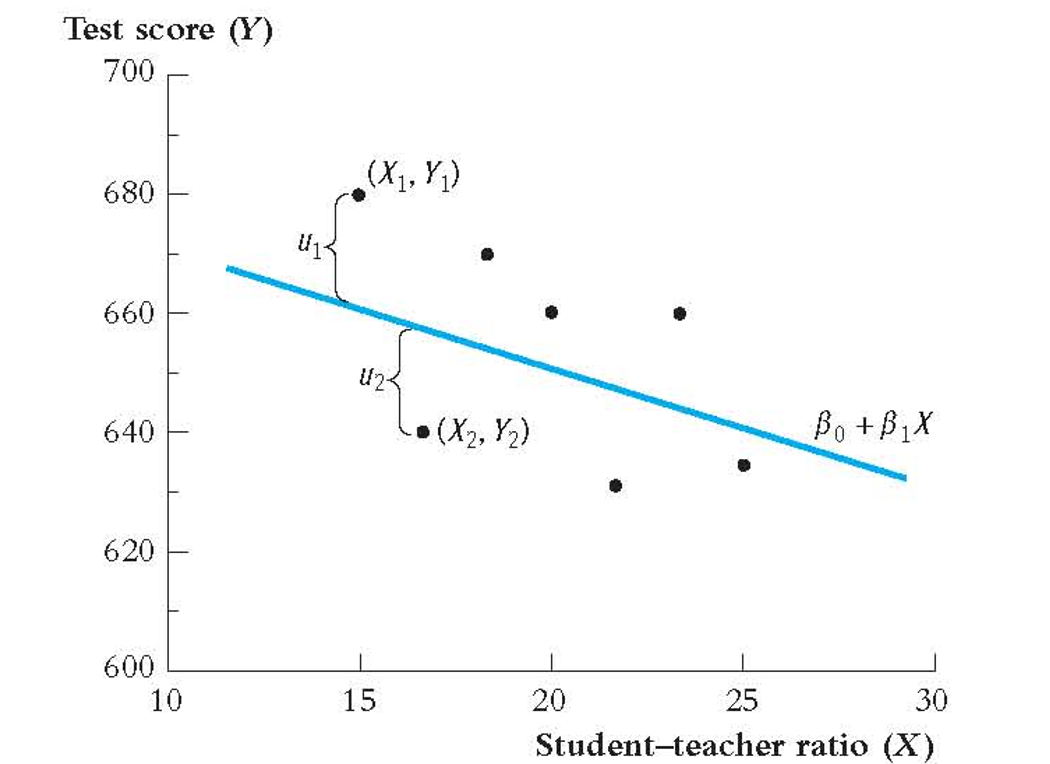
\includegraphics[width=30em]{CS_line.png}
%\end{center}
%\end{frame}


\begin{frame}{Derivation of Bivariate Linear Regression Estimator}
\[
	y_i = \beta_0 + \beta_1 x_i + \varepsilon_i
	\]

\[
		SSR\left(b_0,b_1\right) = \sum_{i=1}^{n} e_i \left(b_0,b_1\right)^2  =  \sum_{i=1}^{n} \left(y_i - b_{0} - b_{1} x_{i}\right)^{2} 
	\]


	\begin{itemize}
		\item (On board) What are the OLS estimates of $\left(\beta_0,\beta_1\right)$?
	\end{itemize}
\end{frame}

\begin{frame}{OLS Estimator}
	\begin{itemize}
\item The OLS estimates are:
\begin{align*}
\hat{b}_1 &=\frac{\sum\limits_{i=1}^n(x_i-\bar{x})(y_i-\bar{y})}{\sum\limits_{i=1}^n(x_i-\bar{x})^2}=\frac{s_{xy}}{s_{x}^{2}} \\
\\
\hat{b}_0 & = \bar{y} - \hat{b}_1 \bar{x}
\end{align*}
where $s_{x}^{2}$ refers to the sample variance of $x$ and $s_{xy}$ refers to the sample covariance of $x$ and $y$.

	\end{itemize}
\end{frame}


\begin{frame}{Using the OLS Estimator}
\begin{itemize}
\item Now let's go ahead and actually use the OLS estimator.
\medskip
\item Suppose Alice has a test score of 6 and class size of 15; Bob has a test score of 3 with a class size of 20. 
\medskip
\item Our data is:
\begin{itemize}
\item Alice: $(y_1,x_1)=(6,15)$
\item Bob: $(y_2,x_2)=(3,20)$
\end{itemize}

\item Note that this is  a ridiculously small sample size (the smallest we could have and still solve for the OLS estimator). 
\end{itemize}
\end{frame}

\begin{frame}{Implementing the OLS Estimator}
\begin{itemize}
\item (On board) Find the OLS estimator for $\beta_0$ and $\beta_1$ for the data $(y_1,x_1)=(6,15)$ and $(y_2,x_2)=(3,20)$
\medskip

\item Formulas:
\begin{align*}
\hat{b}_1 &=\frac{\sum\limits_{i=1}^n(x_i-\bar{x})(y_i-\bar{y})}{\sum\limits_{i=1}^n(x_i-\bar{x})^2}=\frac{s_{xy}}{s_{x}^{2}} \\
\hat{b}_0 & = \bar{y} - \hat{b}_1 \bar{x}
\end{align*}

\item You will never have to do this algebra yourself. It becomes very cumbersome with lots of observations and with lots of regressors,
which we now turn to.

\end{itemize}
\end{frame}


\begin{frame}{Multiple Linear Regression}
\begin{itemize}
	\item Let's return to the multiple linear regression setting (multiple regressors):
	\begin{equation*}
		{\bf y}= {\bf X} \boldsymbol{\beta} + \boldsymbol{\varepsilon},
	\end{equation*}

	\item We can write the sum of squared residuals as follows:\[
	SSR\left({\bf b}\right) = {\bf e} \left({\bf b}\right) '  {\bf e} \left({\bf b}\right) = \left({\bf y} - {\bf X}{\bf b}\right)'\left({\bf y} - {\bf X}{\bf b}\right) = {\bf y}'{\bf y} - 2{\bf y}'{\bf X}{\bf b} + {\bf b}' {\bf X}'{\bf X}{\bf b} 
\]


	\item The necessary condition for a minimum:\[
	\frac{\partial SSR\left({\bf b}\right)}{\partial {\bf b}} = - 2 {\bf X}' {\bf y} + 2 {\bf X}'{\bf X} {\bf b} = {\bf 0} 
	\]

	\item Recalling the rules (the second for symmetric ${\bf A}$, such as ${\bf X}'{\bf X}$):\[
\frac{\partial{\bf u}'{\bf v}}{\partial{\bf v}}={\bf u}\qquad\qquad\frac{\partial{\bf v}'{\bf A}{\bf v}}{\partial{\bf v}}=2{\bf A}{\bf v}
\]

\end{itemize}
\end{frame}


\begin{frame}{The OLS Formula}
\begin{itemize}
	\item The necessary condition for a minimum:\[
	\frac{\partial SSR\left({\bf b}\right)}{\partial {\bf b}} = - 2 {\bf X}' {\bf y} + 2 {\bf X}'{\bf X} {\bf b} = {\bf 0} 
	\]

	\item Thus, ${\bf b}$ must satisfy\[
	{\bf X}'{\bf X} {\bf b} =  {\bf X}' {\bf y} 
	\]


	\item Assuming ${\bf X}'{\bf X}$ is invertible (be careful!), we have\[
	{\bf b}_{OLS} \equiv  \left({\bf X}'{\bf X}\right)^{-1} {\bf X}' {\bf y} 
	\]

	\item Note the similarity to the bivariate least squares estimator. 

\end{itemize}
\end{frame}


\begin{frame}{Full Rank and Identification}
\begin{itemize}
	\item The invertibility of ${\bf X}'{\bf X}$ is not guaranteed in general, but
	it is implied by the full rank condition: $\operatorname{rank}\left({\bf X}\right) = K$.

	\item When ${\bf X}$ does not have full rank, neither does ${\bf X}'{\bf X}$, and \[
	{\bf X}'{\bf X} {\bf b} =  {\bf X}' {\bf y} 
	\]
	can be solved by multiple values of ${\bf b}$. 

	\item Linear algebra review: when a square matrix ${\bf A}$ is not invertible, 
	it has a non-trivial nullspace. This means that \[
	{\bf A} {\bf b} =  {\bf 0}
	\]
	can be solved by multiple vectors ${\bf b}$. This implies that, for any ${\bf c} $,
	\[
	{\bf A} {\bf b} =  {\bf c} 
	\]
	also has multiple solutions if it has at least one solution. 
	

\end{itemize}
\end{frame}


\begin{frame}{Properties of Residuals}
\begin{itemize}
	\item Let ${\bf e} $ denote the vector of OLS residuals, and consider \[
		{\bf X}' {\bf e} = {\bf X}' \left({\bf y} - {\bf X} {\bf b}_{OLS} \right) 
	\]
	\item Substituting in the OLS formula, 
 \[
		{\bf X}' {\bf e} = {\bf X}' \left({\bf y} - {\bf X} \left({\bf X}'{\bf X}\right)^{-1} {\bf X}' {\bf y} \right) 
	\]

\item This simplifies to 
 \[
		{\bf X}' {\bf e} = {\bf X}' {\bf y} -  {\bf X}'{\bf X}\left({\bf X}'{\bf X}\right)^{-1}{\bf X}' {\bf y}  = {\bf X}' {\bf y} -  {\bf X}' {\bf y}  = {\bf 0}
	\]

	\item This implies that (1) the OLS residuals sum to zero, given that one of the regressors is a constant, and
	(2) the OLS residuals are orthogonal to (and, given the constant, uncorrelated with) every regressor. Intuitively: there is no variation left in ${\bf e} $
	 that can be explained by ${\bf X}$.
	
\end{itemize}
\end{frame}


\begin{frame}{Method of moments preview}
\begin{itemize}
	\item Exercise: show that ${\bf b}_{OLS}$ is the unique value of ${\bf b}$ satisfying 
	\[
		{\bf X}' \left({\bf y} - {\bf X} {\bf b}  \right) ={\bf 0}
	\]
	given that ${\bf X}$ is full rank.

	\medskip
	\item Note that ${\bf X}$ is full rank $\Rightarrow$ ${\bf X}'{\bf X}$ is full rank.

	\medskip 
	\item Given this uniqueness result, we could use this condition to define the OLS estimator 
	instead of the least squares definition. 
	This previews {\bf method of moments} estimators, which we will discuss later.
	
\end{itemize}
\end{frame}

%\begin{frame}{Projections}
%\begin{itemize}
%	\item 
%\end{itemize}
%\end{frame}


%\begin{frame}{Idempotence}
%\begin{itemize}
%	\item 
%\end{itemize}
%\end{frame}


\begin{frame}{Multiple Regression Coefficients}
	\begin{itemize}
\item We saw that for a bivariate regression, the slope on the regressor is given by
\[
\hat{b}_1 =\frac{s_{xy}}{s_{x}^{2}} 
\]

\medskip
\item Does it follow that, with multiple regressors, the coefficient on the $k$th regressor is
\[
\hat{b}_k =\frac{s_{x_{k}y}}{s_{x_{k}}^{2}} ?
\]

\medskip
\item If not, under what conditions?

\end{itemize}
\end{frame}


\begin{frame}{Silly Example}
	\begin{itemize}
	\item Consider the following model of rectangular painting area:\[
	\ln A_{i} = \beta_0 + \beta_{1} \ln W_{i} + \beta_{2} \ln H_{i} + \varepsilon_{i}
	\]
	where 
	\begin{itemize}
		\item $W_{i}$ is the painting $i$'s width
		\item $H_{i}$ is the painting $i$'s height
		\item $A_{i}$ is the painting $i$'s area, $A_{i} =W_{i} \cdot H_{i} $
		\item $\varepsilon_i$ is measurement error in painting $i$'s area
	\end{itemize}

	\medskip
	\item What should the $\beta$'s be in theory (i.e., given what you know about geometry)?
\end{itemize}
\end{frame}



\begin{frame}{Silly Example II}
	\begin{itemize}
	\item Suppose $\ln W_i$ and $\ln H_i$ are correlated in the population (naturally)\[
\left(\begin{array}{c}
\ln W_{i}\\
\ln H_{i}
\end{array}\right)\sim\mathcal{N}\left(\left(\begin{array}{c}
\mu_w\\
\mu_h
\end{array}\right),\left(\begin{array}{cc}
\sigma_{w}^{2} & \sigma_{wh}\\
\sigma_{wh} & \sigma_{h}^{2}
\end{array}\right)\right)
\]
	\smallskip
	\item Then, since $\ln A_{i} = \ln W_{i} + \ln H_{i} + \varepsilon_{i}$ with $\varepsilon_{i}$ independent of $\left(W_{i},H_{i}\right)$,\[
	\begin{array}{ll}
	\Cov\left( \ln A_{i}, \ln W_{i}\right) & = \Cov\left(\ln W_{i} + \ln H_{i} + \varepsilon_{i}, \ln W_{i}\right) \\
	& = \Var\left( \ln W_{i}\right) + \Cov\left(\ln W_{i}, \ln H_{i}\right) 
	\end{array}
	\]

	\smallskip
	\item Finally, \[
\hspace*{-.5cm}\frac{\Cov\left(\ln A,\ln W\right)}{\Var\left(\ln W\right)}=\frac{\Var\left(\ln W\right)+\Cov\left(\ln H,\ln W\right)}{\Var\left(\ln W\right)}=1+\frac{\Cov\left(\ln H,\ln W\right)}{\Var\left(\ln W\right)}
\]
\end{itemize}
\end{frame}


\begin{frame}{Silly Example III}
	\begin{itemize}
	\item In a bivariate regression of $\ln A$ on $\ln W$ (omitting $\ln H$), recall the slope would be given by \[
	\hspace*{-.5cm}\frac{\Cov\left(\ln A,\ln W\right)}{\Var\left(\ln W\right)}=1+\frac{\Cov\left(\ln H,\ln W\right)}{\Var\left(\ln W\right)},
	\]
	so the term $\frac{\Cov\left(\ln H,\ln W\right)}{\Var\left(\ln W\right)}$ represents bias. 

	\smallskip
	\item Implication: if the OLS coefficients in a multiple regression had the same formula 
	as the coefficients in a bivariate regression, there would be bias. 

	\smallskip
	\item Exception: if the regressors $\ln H$ and $\ln W$ are uncorrelated, there will be no bias above, and
	OLS with multiple regressors delivers the same coefficients as if we ran a bivariate regression with each
	of the regressors separately. 

	\smallskip
	\item This example also makes a point about omitted variables bias: if height is unobserved, the regression
	of $\ln A$ on only $\ln W$ will deliver the biased coefficient above.

\end{itemize}
\end{frame}


\begin{frame}[fragile]{Silly Example: check it by simulation}
The virtue of a silly example: we \alert{know} the truth ($\beta_1 = \beta_2 = 1$), so we can
watch the bias appear and disappear.
\begin{lstlisting}
library(MASS)
Sigma <- matrix(c(1, 0.6, 0.6, 1), 2, 2)     # corr(log W, log H) = 0.6
wh    <- mvrnorm(10000, mu = c(1, 1), Sigma)
logW  <- wh[,1]; logH <- wh[,2]
logA  <- logW + logH + rnorm(10000, sd = 0.1) # true betas = (1, 1)

coef(lm(logA ~ logW))         # short regression: slope approx 1.6 (biased!)
coef(lm(logA ~ logW + logH))  # long regression:  both approx 1 (as they should be)
\end{lstlisting}
\begin{itemize}
	\item The short-regression slope is $1 + \frac{\Cov(\ln H, \ln W)}{\Var(\ln W)} = 1.6$ --- exactly the formula from the previous slide.
	\item This is the template for the whole course: \alert{derive} the bias with the operator rules, then \alert{simulate} to confirm.
\end{itemize}
\end{frame}

\begin{frame}{Silly Example IV}

	\[
	{\bf b}_{OLS} \equiv  \left({\bf X}'{\bf X}\right)^{-1} {\bf X}' {\bf y} 
	\]


	\begin{itemize}
	\item Indeed, OLS with multiple regressors does not deliver 
	the bivariate regression coefficient $s_{x_{k}y}/s_{x_{k}}^{2}$ for each regressor $x_{k}$
	(except in the case of orthogonal regressors)

	\bigskip
	\item To gain some intuition for what this formula is doing, let's consider the $ \left({\bf X}'{\bf X}\right)$
	and ${\bf X}' {\bf y} $ pieces separately in the context of the silly model of painting area.


\end{itemize}
\end{frame}






\begin{frame}{Silly Example V}


	\begin{itemize}
	\item Suppose that $w_{i}=\ln W_{i}-\mu_{w}$, $h_{i}=\ln H_{i}-\mu_{h}$, and $y_{i}=\ln A_{i}-\mu_{a}$


	\item Let ${\bf X}=\left[{\bf w}\quad{\bf h}\right]$ (an $n\times 2$ matrix, no constant needed since everything is de-meaned)

	\item It follows that 
\[
{\bf X}'{\bf X}=\left(\begin{array}{cc}
\sum_{i} w_{i}^{2} & \sum_{i} w_{i}h_{i}\\
\sum_{i} w_{i}h_{i} & \sum_{i} h_{i}^{2}
\end{array}\right)
\]
Note: if we multiply that by $n^{-1}$, we have the sample analog of the
covariance matrix. 
	
\end{itemize}
\end{frame}

\begin{frame}{Silly Example VI}

	\begin{itemize}
	\item Similarly,
\[
{\bf X}'{\bf y}=\left(\begin{array}{c}
\sum_{i} w_{i}y_{i}\\
\sum_{i} h_{i}y_{i}
\end{array}\right),
\]
is the sample covariance of ${\bf x}_{i}$ and $y_{i}$
(times $n$). 

\smallskip
\item Therefore, we have
\[
{\bf b}_{OLS}=\left({\bf X}'{\bf X}\right)^{-1}{\bf X}'{\bf y}=\left(n^{-1}{\bf X}'{\bf X}\right)^{-1}\left(n^{-1}{\bf X}'{\bf y}\right)={\bf S}_{xx}^{-1}{\bf s}_{xy}
\]
where ${\bf S}_{xx}$ is the sample covariance matrix of ${\bf x}_{i}$
and ${\bf s}_{xy}$ is the vector of sample covariances of ${\bf x}_{i}$ with $y_{i}$. 

\end{itemize}
\end{frame}


\begin{frame}{Silly Example VII}

\[
{\bf b}_{OLS}={\bf S}_{xx}^{-1}{\bf s}_{xy}
\]

\begin{itemize}
	\item The population moments for the model of painting areas are \[
\Var\left({\bf x}_{i}\right)=\left(\begin{array}{cc}
\sigma_{w}^{2} & \sigma_{wh}\\
\sigma_{wh} & \sigma_{h}^{2}
\end{array}\right)\qquad\qquad \Cov\left({\bf x}_{i},y_{i}\right)=\left(\begin{array}{c}
\sigma_{w}^{2}+\sigma_{wh}\\
\sigma_{h}^{2}+\sigma_{wh}
\end{array}\right)
\]

\item Note that 
\[
\Var\left({\bf x}_{i}\right)^{-1}=\frac{1}{\sigma_{w}^{2}\sigma_{h}^{2}-\sigma_{wh}^{2}}\left(\begin{array}{cc}
\sigma_{h}^{2} & -\sigma_{wh}\\
-\sigma_{wh} & \sigma_{w}^{2}
\end{array}\right)
\]

\item With some algebra, the population-moments version of OLS gives us the right coefficients:
\[
\Var\left({\bf x}_{i}\right)^{-1}\Cov\left({\bf x}_{i},y_{i}\right)=\left(\begin{array}{c}
1\\
1
\end{array}\right)
\]
\end{itemize}
\end{frame}







\begin{frame}{The Frisch-Waugh Theorem I}
\begin{itemize}
	\item Think about separating $ {\bf X}$ into two sub-matrices:\[
	 {\bf X} =  \left[{\bf X}_{1}\quad  {\bf X}_2 \right],
	\]
	with \[
	{\bf y} = {\bf X}_{1} \boldsymbol{\beta}_{1} +  {\bf X}_{2} \boldsymbol{\beta}_{2} + \boldsymbol{\varepsilon}
	\]
\end{itemize}

\begin{block}{Frisch-Waugh Theorem}
In the OLS regression of ${\bf y} $ on $\left[{\bf X}_{1},  {\bf X}_2 \right]$,
the subvector ${\bf b}_{2}$ of coefficients on ${\bf X}_{2}$ equals the coefficients from regressing
the residuals of ${\bf y}$ on ${\bf X}_{1}$ on the residuals of ${\bf X}_{2}$ on ${\bf X}_{1}$:
\[
{\bf b}_{2} = \left({\bf X}_{2}'{\bf M}_{1}{\bf X}_{2}\right)^{-1}{\bf X}_{2}'{\bf M}_{1}{\bf y},
\qquad {\bf M}_{1} = {\bf I} - {\bf X}_{1}\left({\bf X}_{1}'{\bf X}_{1}\right)^{-1}{\bf X}_{1}'.
\]

\end{block}
\end{frame}

\begin{frame}{The Frisch-Waugh Theorem II}
\begin{itemize}
	\item In other words, let's start by regressing ${\bf y} $ on ${\bf X}_{1}$.
	Let's label the residuals from this regression ${\bf y}^{*} = {\bf M}_{1}{\bf y}$.

	\item Let's also regress ${\bf X}_{2}$ on ${\bf X}_{1}$ 
	(think about regressing each column of ${\bf X}_{2}$ on ${\bf X}_{1}$).
	Let's label the residuals from this regression ${\bf X}^{*}_{2} = {\bf M}_{1}{\bf X}_{2}$.

	\item If we regress ${\bf y}^{*}$ on ${\bf X}^{*}_{2}$, we get the same
	coefficient on ${\bf X}^{*}_{2}$ that we would have had in the full
	regression of  ${\bf y} $ on $\left[{\bf X}_{1},  {\bf X}_2 \right]$.

	\item An implication is that
	the coefficient on each variable can be thought of as the effect
	of that variable after controlling for all the other variables. Thus,
	OLS coefficients are sometimes called {\bf partial regression coefficients}.

\end{itemize}
\end{frame}



\begin{frame}{The Frisch-Waugh Theorem III}
\begin{itemize}
	\item Bivariate linear regression is easy to visualize (scatter plot with a line running through).
	Frisch-Waugh tells us how we can visualize the effect of a single variable from a multiple
	regression.

	\medskip
	\item One implication of Frisch-Waugh is that, if we de-mean all the variables and then 
	run a regression with the de-meaned variables (but leaving out the constant term in ${\bf X}$),
	we will get the same coefficients on all the variables.
	\begin{itemize}
		\item Exercise: given the Frisch-Waugh theorem, show this formally. 
	\end{itemize}
\end{itemize}
\end{frame}



\begin{frame}{Units and Coefficients}
\begin{itemize}
	\item Recalling that $\E\left[{\bf y}|{\bf X}\right] = {\bf X} \boldsymbol{\beta}$, a natural interpretation	of
	the coefficients is 
	is \[
	\beta_k = \frac{\partial }{\partial x_{k,i}}\E\left[y_i |{\bf X}\right]
	\]
	
	\item In simple linear regression, it's easy to see that re-scaling (changing the units
	of $x$) will rescale the parameter estimates in the opposite way:\[
		\hat{b}_1 =\frac{\sum\limits_{i=1}^n(x_i-\bar{x})(y_i-\bar{y})}{\sum\limits_{i=1}^n(x_i-\bar{x})^2}
	\]
 	The same is true in the multiple regression framework (Frisch-Waugh makes this easier to see). 

	\medskip
	\item Exercise: if the regressor $x$ in a bivariate regression
	is the log of a variable, show that rescaling the original variable does not
	affect $\hat{b}_1 $. What about $\hat{b}_0$? 
\end{itemize}
\end{frame}




\begin{frame}{Goodness of Fit}
\begin{itemize}
	\item The {\bf total sum of squares}, or the {\bf total variation} in the dependent variable:\[
	SST = \left({\bf y} - {\bf i} \overline{y} \right)' \left({\bf y} - {\bf i} \overline{y} \right) = {\bf y}'{\bf M}_{0}{\bf y}
	\]
	where ${\bf i}$ is an $n\times 1$ vector of ones and ${\bf M}_{0} = {\bf I} - n^{-1}{\bf i}{\bf i}'$ de-means a vector.

	\smallskip
	\item The dependent variable decomposes into a prediction and a residual:\[
	{\bf y} = {\bf X} {\bf b}_{OLS} + {\bf e} =  \widehat{{\bf y}} + {\bf e}
	\]
where $\widehat{{\bf y}} = {\bf X} {\bf b}_{OLS}$ is the prediction or {\bf fitted value} of ${\bf y}$. 

	\smallskip
	\item We can think about decomposing the variation in $y$ into variation in $ \widehat{{\bf y}}$ and ${\bf e}$.
	Intuitively, we want the variation in  $ \widehat{{\bf y}}$ to account for as much as possible
\end{itemize}
\end{frame}



\begin{frame}{Coefficient of Determination}
\begin{itemize}
	\item The variation in $y$ splits cleanly into explained and unexplained pieces
	when ${\bf X}$ includes a constant
	(this is the \alert{law of total variance} from Lecture 1, in sample form):\[
	\underbrace{SST}_{\text{total}} = \underbrace{SSE}_{\text{explained}} + \underbrace{SSR}_{\text{residual}},
	\qquad SSE = \widehat{{\bf y}}'{\bf M}_{0}\widehat{{\bf y}}, \quad SSR = {\bf e}'{\bf e}
	\]
	(The matrix version of this decomposition: Hansen 3.13.)

	\smallskip
	\item The coefficient of determination is the proportion of the variation in the dependent variable
	explained by the model:\[
	R^{2} = \frac{SSE}{SST}
	= 1 -  \frac{{\bf e}'{\bf e}}{{\bf y}'{\bf M}_{0}{\bf y}}
\]

	\smallskip
	\item $R^{2}$ is a measure of goodness of fit that never goes down as we add more regressors. It doesn't 
	tell us whether it's ``worth it'' to add a new regressor to the model. (Later we will talk about why overfitting
	can be bad in finite samples.)
\end{itemize}
\end{frame}


\begin{frame}{Adjusted $R^{2}$}
\begin{itemize}
	\item Adding a regressor can only lower ${\bf e}'{\bf e}$, so $R^{2}$ can only rise (weakly).
	It is useless for deciding whether the regressor belongs in the model.

	\medskip
	\item {\bf Adjusted} $R^{2}$ charges a price for each parameter by comparing
	variances rather than sums of squares:\[
	\overline{R}^{2} 	= 1 -  \frac{{\bf e}'{\bf e}/\left(n-K\right)}{{\bf y}'{\bf M}_{0}{\bf y}/\left(n-1\right)}
	\]

	\medskip
	\item Each new regressor shrinks ${\bf e}'{\bf e}$ in the numerator but also shrinks its
	degrees of freedom $n-K$, so $\overline{R}^{2}$ can fall.

	\medskip
	\item It can even go negative. Treat it as a rule of thumb, not a model selection
	criterion.
\end{itemize}
\end{frame}




\begin{frame}{Finite Sample Properties}
\begin{itemize}
	\item Given assumptions (1)-(3), homoscedasticity, and normal error terms, \[
	{\bf b}_{OLS} | {\bf X} \sim \mathcal{N}\left(\boldsymbol{\beta},\sigma^{2} \left({\bf X}'{\bf X}  \right)^{-1} \right)
	\]

	\item Unbiasedness is a two-line operator derivation. Substitute ${\bf y}$ into the OLS formula:
	\begin{align*}
		{\bf b}_{OLS} &= \left({\bf X}'{\bf X}\right)^{-1}{\bf X}'\left({\bf X}\boldsymbol{\beta} + \boldsymbol{\varepsilon}\right)
		= \boldsymbol{\beta} + \left({\bf X}'{\bf X}\right)^{-1}{\bf X}'\boldsymbol{\varepsilon}\\
		\E\left[{\bf b}_{OLS}|{\bf X}\right] &= \boldsymbol{\beta} + \left({\bf X}'{\bf X}\right)^{-1}{\bf X}'\underbrace{\E\left[\boldsymbol{\varepsilon}|{\bf X}\right]}_{=0 \text{ (strict exog.)}} = \boldsymbol{\beta}
	\end{align*}

	\item Note: unbiasedness and the variance expression
	do not require normal error terms, but it would be hard to say what the finite sample
	distribution is, exactly, without normality.

\end{itemize}
\end{frame}




\begin{frame}{Standard Errors}

\[
	{\bf b}_{OLS} | {\bf X} \sim \mathcal{N}\left(\boldsymbol{\beta},\sigma^{2} \left({\bf X}'{\bf X}  \right)^{-1} \right)
	\]

\begin{itemize}
	\item $\sigma^{2} \left({\bf X}'{\bf X}  \right)^{-1}$ is the covariance matrix of the parameter estimates
	-- it tells us how precise ${\bf b}_{OLS}$ is as an estimate of $\boldsymbol{\beta}$.

	\item The diagonal elements of $\sigma^{2} \left({\bf X}'{\bf X}  \right)^{-1}$ are the variances of each of
	the parameter estimates. The square roots of those are {\bf standard errors}. Note that standard
	errors are standard deviations of the distribution of an estimator. 

	\item The off-diagonal elements of $\sigma^{2} \left({\bf X}'{\bf X}  \right)^{-1}$ are also important
	(especially when we get to hypothesis testing).
	They indicate whether two parameter estimates are correlated.

\end{itemize}
\end{frame}

\begin{frame}{Estimating Standard Errors}

\[
	{\bf b}_{OLS} | {\bf X} \sim \mathcal{N}\left(\boldsymbol{\beta},\sigma^{2} \left({\bf X}'{\bf X}  \right)^{-1} \right)
	\]

\begin{itemize}
	\item $\left({\bf X}'{\bf X}  \right)^{-1}$ is just data, but $\sigma^{2}$ must be estimated (recall that it's the 
	variance of the normally distributed error terms). 

	\item Intuitively, the residuals are estimates of the error terms, so the sample variance of residuals
	is what we use to estimate $\sigma^{2}$:\[
	s^{2} = \frac{{\bf e}'{\bf e}}{n-K}
	\]

	\item Similar to how the unbiased estimator of the variance of a random variable with unknown mean requires us to divide
	by $n-1$, here we have to divide by $n-K$, where $K$ is the number of parameters being estimated. 

	
\end{itemize}
\end{frame}


\begin{frame}{Mean-squared error}
\begin{itemize}
	\item Consider a parameter vector $\boldsymbol{\gamma}$ and consider
	${\bf x}'\boldsymbol{\gamma}$ as a predictor of $y$. 

	\medskip
	\item The {\bf mean squared error} of this predictor is\[
	MSE\left(\boldsymbol{\gamma}\right) = \E\left[\left( y - {\bf x}' \boldsymbol{\gamma}\right)^{2}\right]
	\]

	\item This can be written\[
	MSE\left(\boldsymbol{\gamma}\right) = \E\left[ \left(y - \E\left[y | {\bf x}\right]\right)^{2}\right] + \E\left[  \left(\E\left[y | {\bf x}\right]- {\bf x}' \boldsymbol{\gamma}\right)^{2} \right]
	\]
	(check this by expanding and applying the law of iterated expectations)

	\item Result: the minimizer is $\boldsymbol{\gamma}^{*} = \E\left[{\bf x}{\bf x}'\right]^{-1}\E\left[{\bf x}y\right]$, and OLS is its
	sample analog. By the decomposition, ${\bf x}'\boldsymbol{\gamma}^{*}$ is also the best linear approximation to $\E\left[y|{\bf x}\right]$.
	This does not require normality of the error terms. (Good operator practice: expand the square and apply
	the law of iterated expectations.)

\end{itemize}
\end{frame}


\begin{frame}{Gauss-Markov Theorem}

\begin{block}{Gauss-Markov Theorem}
In the linear regression model with homoscedastic errors, the OLS estimator 
is the {\bf best linear unbiased estimator} (BLUE).
\end{block}

\begin{itemize}
	\item ``Best'' means lowest variance in the matrix sense: $\Var\left[\widetilde{{\bf b}}|{\bf X}\right] - \Var\left[{\bf b}_{OLS}|{\bf X}\right]$ is positive semidefinite for any other linear unbiased $\widetilde{{\bf b}}$

	\item Normally distributed error not assumed here

	\item If error terms are not homoscedastic, OLS is still unbiased given strict
	exogeneity, but lower-variance estimators are possible (see: Generalized Least Squares)

	\item We won't prove this (Hansen 4.7). In practice the modern response to
	heteroskedasticity is not a ``better'' estimator but \alert{robust standard errors}
	for OLS --- next lecture.

\end{itemize}
\end{frame}


\begin{frame}{Generalized Least Squares}
\begin{itemize}
	\item The proof that OLS is unbiased did not rely on homoskedasticity. OLS
	is ``LUE'' even without homoskedasticity. OLS is only {\bf B}LUE (minimal variance) with homoskedasticity.

	\smallskip
	\item Without homoskedasticity, but maintaining our other assumptions, {\bf Generalized
		Least Squares} is BLUE. That is, suppose,\[
	\Var\left[\boldsymbol{\varepsilon} | {\bf X} \right] = \boldsymbol{\Omega}
	\]
	then the BLUE estimator is \[
	{\bf b}_{GLS} = \left({\bf X}'\boldsymbol{\Omega}^{-1}{\bf X}\right)^{-1} {\bf X}' \boldsymbol{\Omega}^{-1}{\bf y} .
	\]
	
	\smallskip
	\item To implement GLS, note that $\boldsymbol{\Omega}$ must be estimated ({\bf Feasible Generalized
		Least Squares}). In contrast, OLS estimates the $\boldsymbol{\beta}$ parameters without needing to know or estimate
		anything about variances; $\sigma^2$ is only needed to quantify standard errors. 
\end{itemize}
\end{frame}



\begin{frame}{Endogeneity}
\[
	{\bf b}_{OLS} = \left({\bf X}'{\bf X}\right)^{-1} {\bf X}' {\bf y} = \boldsymbol{\beta}  + \left({\bf X}'{\bf X}\right)^{-1} {\bf X}' \boldsymbol{\varepsilon}
	\]
\begin{itemize}
		\item Note that our argument for OLS being unbiased involved a step where we argue that \[
	\E\left[\left({\bf X}'{\bf X}\right)^{-1} {\bf X}' \boldsymbol{\varepsilon} | {\bf X}\right] ={\bf 0}
	\]
	thanks to strict exogeneity.

	\medskip
	\item If one of the regressors is correlated with $\varepsilon$, strict exogeneity is violated, and this term will cause bias. 

\end{itemize}
\end{frame}


\begin{frame}{Omitted Variables Bias}
\begin{itemize}
	\item Suppose the econometrician only observes regressors ${\bf X} $, but the true model is\[
			{\bf y}= {\bf X} \boldsymbol{\beta} + {\bf z} \gamma + \boldsymbol{\varepsilon},
	\]

	\item The OLS estimator will equal\[
	{\bf b}_{OLS} = \left({\bf X}'{\bf X}\right)^{-1} {\bf X}' {\bf y} = \boldsymbol{\beta}  + \left({\bf X}'{\bf X}\right)^{-1} {\bf X}' {\bf z} \gamma + \left({\bf X}'{\bf X}\right)^{-1} {\bf X}' \boldsymbol{\varepsilon}
	\]

	\item The last term is mean zero given the strict exogeneity assumption.

	\item The second term is $\gamma$ times the coefficients from regressing ${\bf z}$ on ${\bf X}$, so it is
	nonzero when ${\bf X}$ and ${\bf z}$ are correlated; i.e., if $ {\bf X}' {\bf z} \ne {\bf 0}$.

	\item Implication:  correlation between omitted variables and the observed regressors makes OLS biased.

	
\end{itemize}
\end{frame}







\begin{frame}{Bias with multiple variables}
\begin{itemize}
		\item<1-> Consider a model with two variables:\[
			y_i = \beta_0 + \beta_1 x_{1,i} + \beta_2 x_{2,i} + \varepsilon_i,
		\]
		and suppose that
		\begin{align*}
			x_{1,i} =& u_{1,i} + u_{3,i} + \varepsilon_i  \\
			x_{2,i} =& u_{2,i} + u_{3,i}
		\end{align*}		
		where the $u$'s and $\varepsilon$ are all independently distributed. 
		
		\item<1-> We know that OLS will deliver
		a biased (and inconsistent) estimate of $\beta_{1}$, but will OLS still be consistent for $\beta_2$?
		
		\medskip
		\item<2-> No! The correlation between $x_1$ and $x_2$ leads to bias even
		in $\beta_2$.
		\begin{itemize}
			\item<2-> Thus, endogeneity problems are a big deal not only for our variables of interest; endogenous
			control variables can also create problems.
		\end{itemize}
\end{itemize}
\end{frame}


\begin{frame}{Bias with multiple variables II}
\begin{itemize}
		\item Consider ``controlling'' for $x_1$ with the wrong estimate $b_1$ of $\beta_1$:\[
					y_i - b_1 x_{1,i} = \beta_0 + \beta_2 x_{2,i}  + \varepsilon_i + (\beta_1 - b_1) x_{1,i},
\]

\medskip
		\item Given that $b_1 \ne \beta_1$, we get some stuff in the error term:\[
					y_i - b_1 x_{1,i} = \beta_0 + \beta_2 x_{2,i}  + \varepsilon_i + (\beta_1 - b_1) (u_{1,i} + u_{3,i} + \varepsilon_i),
\]
and we now have an endogeneity problem because $x_{2,i} = u_{2,i} + u_{3,i}$ and $u_{3,i}$ is now in the error term.

\medskip
\item Note: we could formalize this intuition using the Frisch-Waugh Theorem. 
\end{itemize}
\end{frame}


\begin{frame}{Irrelevant Variables}
\begin{itemize}
	\item What if we include a variable in ${\bf X}$ that doesn't actually
	affect $y$?

	\smallskip
	\item This can be accommodated in the linear regression framework as
	a regressor that has a coefficient $\beta_{k}=0$.

	\smallskip
	\item Thus, this does not create any bias in the other coefficients, and the 
	expected coefficient on the irrelevant variable is zero.

	\smallskip
	\item However, this can reduce the precision of the estimates of the 
	other coefficients, and it's not generally a good idea to add as many variables
	to a regression as you can ({\bf overfitting}). More on this later. 

	
\end{itemize}
\end{frame}




\begin{frame}{Finite Sample vs. Asymptotic Properties}
\begin{itemize}
	\item It's rare to have small-sample properties of an estimator

	\medskip
	\item Econometric studies typically do Monte Carlo (simulation) studies to learn
	about finite-sample performance of estimators. 

	\medskip
	\item For most estimators, we derive asymptotic properties, i.e., \[
	\sqrt{n} \left({\bf b}_{OLS} - \boldsymbol{\beta}\right) \overset{d}{\to} \mathcal{N}\left({\bf 0}, {\bf V}\right)
	\]

	\item The above statement says that the OLS estimator
	 {\bf converges in distribution} to a normally distributed variable.

	\item Part of that result is that OLS is {\bf consistent}. Formally, consistency means that an estimator
	{\bf converges in probability} to the true value. 
\end{itemize}
\end{frame}



\begin{frame}{Asymptotics: Setup}
\begin{itemize}

	\item Asymptotic analysis refers to analyzing statistics of the data as the number of observations $n$
	grows to infinity (e.g., the central limit theorem).

	\item To do asymptotic analysis, we specify a {\bf data generating process}. 
	
	\item A data generating process describes the distribution of 
	 a sequence of observations $\left({\bf x}_{i},\varepsilon_{i}\right)$ 	for $i=1,2,\dots n$. 


	\item The simplest case is assuming that observations are {\bf independent and identically distributed}
	(i.i.d)

	\item In other settings, the observations are allowed to be correlated, but in a limited way 
	that requires the dependence between ``distant'' observations to go to zero -- see {\bf stationarity}
	and {\bf ergodicity} (e.g., time series, and 	more recently some spatial analysis)

	\item We also need the data to be ``well-behaved'', i.e. $\E\left[{\bf x}_{i} {\bf x}_{i}' \right]$ must have
	full rank and the error terms must have finite variance. 

\end{itemize}
\end{frame}



\begin{frame}{OLS Asymptotic Distribution}
\begin{itemize}
	\item We can use the central limit theorem to show that OLS is asymptotically
	normally distributed. Under homoskedasticity, ${\bf V} = \sigma^{2}\E\left[{\bf x}_{i}{\bf x}_{i}'\right]^{-1}$, so\[
{\bf b}_{OLS}\overset{a}{\sim}\mathcal{N}\left(\boldsymbol{\beta},\frac{\sigma^{2}}{n}\E\left[{\bf x}_{i}{\bf x}_{i}'\right]^{-1}\right)
\]
	where $\overset{a}{\sim}$ means ``approximately distributed as, in large samples'' (shorthand for the $\sqrt{n}$ statement). 

	\item This is just like the finite-sample distribution
	we got with normally distributed error terms.
\end{itemize}
\end{frame}


\begin{frame}{Workbook time}
\begin{center}
{\LARGE \alert{Let's look at the workbook now.}}
\end{center}
\bigskip
\begin{itemize}
	\item Open \texttt{inclass\_session2.Rmd} (in the \texttt{Fall/L3 - Linear Regression} folder of the course repo).
	\item Reproduce the bivariate-normal regression and the Silly Example.
	\item Then work the two problems with a neighbor:
	\begin{enumerate}
		\item Frisch--Waugh with your own hands
		\item A regression is a table of means
	\end{enumerate}
\end{itemize}
\end{frame}


\end{document}